\section{Interrupts}

One of the key features of modern processors is the ability to support \textit{interrupts}.
Unlike many other processor features interrupts are not an arithmetic operation but
rather the ability of a processor to \textit{respond to a event asynchronously}. Events are
unexpected changes that are signaled to the kernel. This chapter will explain in
greater detail what they are and how they work in low level.

\subsection{The different types of interrupts}

Gone are the days where the only instructions CPUs were capable of executing were
purely arithmetic. The engineers behind the chip design in the 80' noticed that
computers are destined to serve a purpose beyond specific mathematical computations,
namely consumer applications.

In
practice this means that a processor may be running a program until an event, such as a pressed
key, \textit{interrupts} the execution of the program and invokes a handler for the event. The
handler runs and upon completion the processor resumes the execution of the program.

\subsection{Hardware}

Most hardware needs to communicate with each other. It is used for \textit{time synchronisation},
\textit{data} and to send \textit{commands}. Devices that are attached to the computer, such as keyboards 
and USB thumb drives as well as coprocessors and hardware located directly on the 
motherboard such as sound cards and the clock, need to be synced, programmed and set up data
exchange. Most of this communication is done via \textit{hardware interrupts}. All these attached
devices are connected to the CPU with a wire called the \textit{interrupt line}. When a device needs the CPU's 
attention it toggles the voltage of the interrupt line. This signals an \textit{interrupt request} to the
processor. The CPU then finishes executing the current instruction and notice the interrupt request and
check which device requested the interrupt. Modern CPU architectures have multiple \textit{interrupt lines}
and each of them can be assigned to a handler. In action this would look like the following:

\begin{figure}[H]
\begin{center}
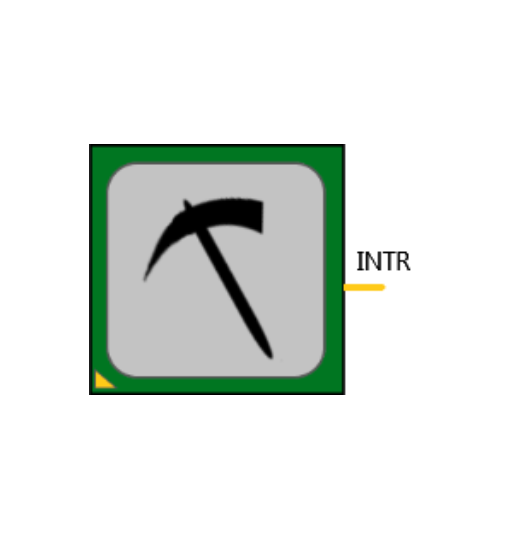
\includegraphics[width=200px]{int0.png}
\caption{A processor is running a regular program.}
\end{center}
\end{figure}

\begin{figure}[H]
\begin{center}
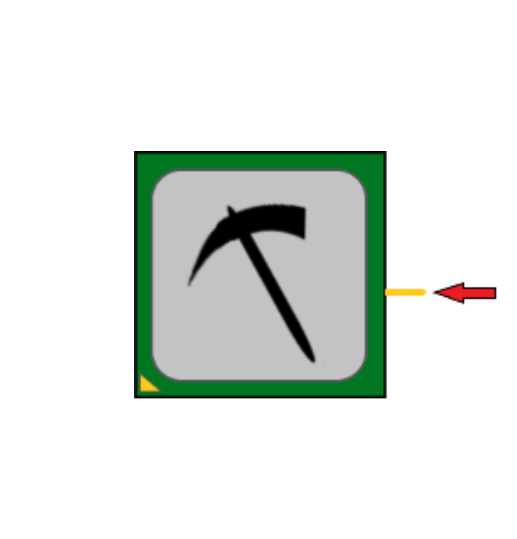
\includegraphics[width=200px]{int1.png}
\caption{Interrupt request line (INTR) gets set high. The CPU finishes the current instruction and notices the interrupt request.}
\end{center}
\end{figure}

\begin{figure}[H]
\begin{center}
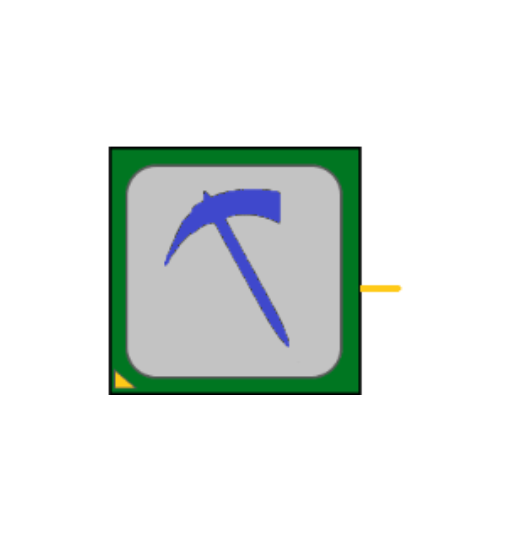
\includegraphics[width=200px]{int2.png}
\caption{The interrupt handler is invoked by the CPU by looking up the handler address from the
interrupt vector table and jumping to this address.}
\end{center}
\end{figure}

\begin{figure}[H]
\begin{center}
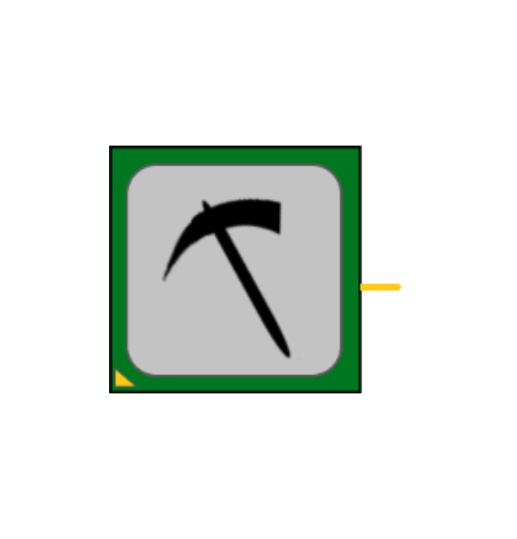
\includegraphics[width=200px]{int3.png}
\caption{The previous program resumes execution once the handler is done. }
\end{center}
\end{figure}


The handler then reprograms the device if needed or performs the data exchange. Hardware 
interrupts allow te processor to do its job and only attend hardware if necessary. This
must be supported by the hardware (interrupt line).

\subsubsection{Interrupts vs Polling}

There are two paradigms used to await input, the aforementioned interrupts and \textit{polling}, 
which is a continous check of hardware status. It is usually implemented in software and 
used in systems that do not support interrupts. This means that a running program must 
frequently check all the attached hardware. The rate of which hardware is checked is called 
the \textit{polling rate}. A high polling rate means that the program must spend a lot of time 
polling and a low latency. This is useful in systems, such as routers, that do not perform 
computationally intensive calculations but need high responsiveness. Most of the time these 
devices \textit{do nothing} until an event occurs. In the case of routers this is an arriving 
internet packet. The device only then stops polling, handle the event i.e. determine 
the packet destination and then reroute the packet accordingly. It then resumes polling once 
again. In the time slice between receiving the packet and rerouting it, the CPU was busy and
was not able to check for another packet. 

\subsection{Software}

\subsection{Interrupt vector table}

Interrupt handlers are essentially \textit{functions} that are automatically executed as soon as an
interrupt occurs. They differ from normal functions because they are not explicitly called.
Processors must know the \textit{address of a function} in order to call them. Interrupt vector
tables (IVTs) are a method to associate interrupts to interrupt handlers. It is essentially an
\textit{array of function pointers}. Interrupts are generally numbered and these numbers are used to look up 
the address of the interrupt handlers. For example, software interrupts are invoked with the `int 
\textless NUMBER\textgreater` instruction. This number is the \textit{interrupt number} and it is used by the CPU to determine 
the address of the handler. The interrupt number is used as an array index. The instruction `int \textit{N}` 
makes the CPU jump to the address pointed to by the IVT's \textit{N}th entry. Some architectures have the IVT
at a fixed location. The earlier versions of x86 processors had the IVT at address 0x0. Every entry
is four bytes long, meaning the address of the `int \textit{N}` handler is at adress `4 \* \textit{N}`. As an exmple,
the `int 0x10` instruction makes the CPU jump to the address that is in the IVT's 0x10's address,
i.e. the address 0x40. \footnote{Interrupts, from: Tutorialspoint, \today  \\ https://www.tutorialspoint.com/embedded\_systems/es\_interrupts.htm}

\subsection{Interrupt requests lines}

Interrupts are also invoked by peripheral devices and they often do not necessarily have a fixed 
interrupt number associated with themselves. In systems with multiple peripheral devices such as for 
example a keyboard and a network adapter it is more practical to have separate interrupt handlers
instead of a single handler. Mapping each peripheral device to its own handler avoids the overhead of 
having to identify which device requested the interrupt. This mapping is done with a coprocessor often
called the \textit{Programmable Interrupt Controller}, PIC for short. An operating system's task is to
\textit{reprogram} the PIC by assigning every peripheral device to its own handler. Reprogramming the PIC also
allows for \textit{prioritized IRQs} i.e. determining which IRQ should be handled first when multiple IRQs 
occur simultaneously. Whenever a new hardware interrupt occurs, the reprogrammed PIC determines
the correct handler, communicate the IRQ number to the processor which invokes said handler. In
modern operating systems with dedicated drivers, the IRQ handler invokes the driver that takes
care of the device reconfiguration or data transfer.
